\documentclass{standalone}
\usepackage{tikz}
\usetikzlibrary{patterns, positioning}


\begin{document}
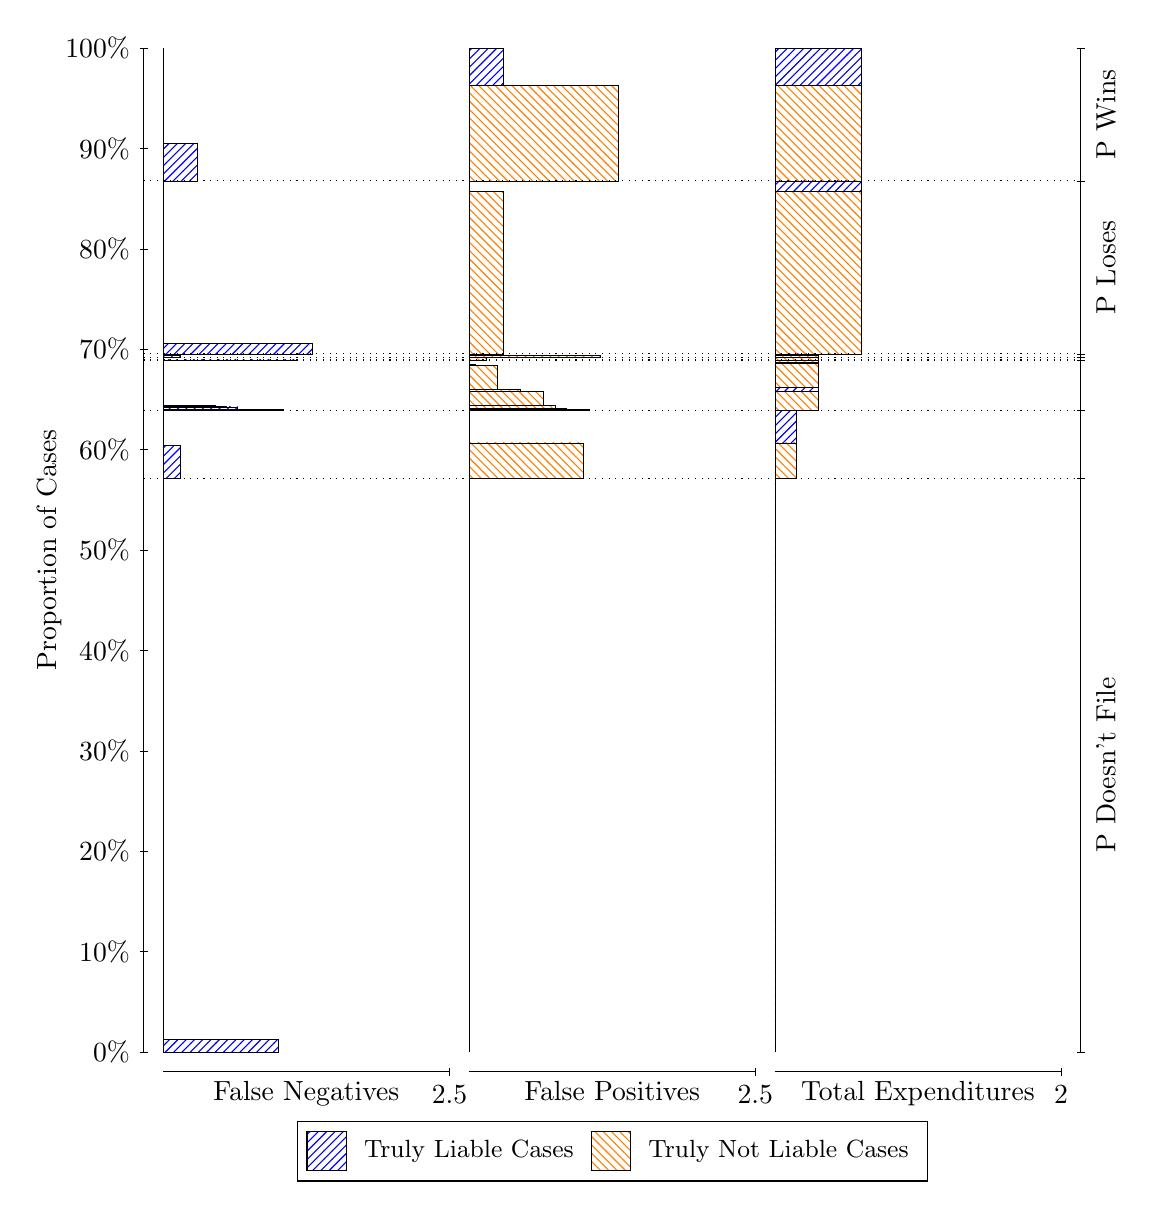
\begin{tikzpicture}
\draw[black, very thin] (1.5,1.75) -- (1.5,14.5);
\node[rotate=90, text=black, anchor=center] at (0.3, 8.125) {Proportion of Cases};
\draw[black, very thin] (1.45,1.75) -- (1.55,1.75);
\node[text=black, anchor=east] at (1.45, 1.75) {0\%};
\draw[black, very thin] (1.45,3.025) -- (1.55,3.025);
\node[text=black, anchor=east] at (1.45, 3.025) {10\%};
\draw[black, very thin] (1.45,4.3) -- (1.55,4.3);
\node[text=black, anchor=east] at (1.45, 4.3) {20\%};
\draw[black, very thin] (1.45,5.575) -- (1.55,5.575);
\node[text=black, anchor=east] at (1.45, 5.575) {30\%};
\draw[black, very thin] (1.45,6.85) -- (1.55,6.85);
\node[text=black, anchor=east] at (1.45, 6.85) {40\%};
\draw[black, very thin] (1.45,8.125) -- (1.55,8.125);
\node[text=black, anchor=east] at (1.45, 8.125) {50\%};
\draw[black, very thin] (1.45,9.4) -- (1.55,9.4);
\node[text=black, anchor=east] at (1.45, 9.4) {60\%};
\draw[black, very thin] (1.45,10.675) -- (1.55,10.675);
\node[text=black, anchor=east] at (1.45, 10.675) {70\%};
\draw[black, very thin] (1.45,11.95) -- (1.55,11.95);
\node[text=black, anchor=east] at (1.45, 11.95) {80\%};
\draw[black, very thin] (1.45,13.225) -- (1.55,13.225);
\node[text=black, anchor=east] at (1.45, 13.225) {90\%};
\draw[black, very thin] (1.45,14.5) -- (1.55,14.5);
\node[text=black, anchor=east] at (1.45, 14.5) {100\%};

\draw[black, very thin] (13.4,1.75) -- (13.4,14.5);
\draw[black, very thin] (13.35,1.75) -- (13.45,1.75);
\node[anchor=west] at (13.35, 1.75) {};
\draw[black, very thin] (13.35,9.0377) -- (13.45,9.0377);
\node[anchor=west] at (13.35, 9.0377) {};
\draw[black, very thin] (13.35,9.9006) -- (13.45,9.9006);
\node[anchor=west] at (13.35, 9.9006) {};
\draw[black, very thin] (13.35,10.538) -- (13.45,10.538);
\node[anchor=west] at (13.35, 10.538) {};
\draw[black, very thin] (13.35,10.574) -- (13.45,10.574);
\node[anchor=west] at (13.35, 10.574) {};
\draw[black, very thin] (13.35,10.615) -- (13.45,10.615);
\node[anchor=west] at (13.35, 10.615) {};
\draw[black, very thin] (13.35,12.814) -- (13.45,12.814);
\node[anchor=west] at (13.35, 12.814) {};
\draw[black, very thin] (13.35,14.5) -- (13.45,14.5);
\node[anchor=west] at (13.35, 14.5) {};

\draw[black, very thin, pattern color=blue, pattern=north east lines] (1.75,1.75) rectangle (3.2033,1.9101);
\draw[black, very thin, pattern color=orange, pattern=north west lines] (1.75,1.9101) rectangle (1.75,9.0377);
\draw[black, very thin, pattern color=blue, pattern=north east lines] (1.75,9.0377) rectangle (1.968,9.4531);
\draw[black, very thin, pattern color=orange, pattern=north west lines] (1.75,9.4531) rectangle (1.75,9.9006);
\draw[black, very thin, pattern color=blue, pattern=north east lines] (1.75,9.9006) rectangle (3.276,9.9081);
\draw[black, very thin, pattern color=blue, pattern=north east lines] (1.75,9.9081) rectangle (3.1307,9.9081);
\draw[black, very thin, pattern color=blue, pattern=north east lines] (1.75,9.9081) rectangle (2.9853,9.9102);
\draw[black, very thin, pattern color=blue, pattern=north east lines] (1.75,9.9102) rectangle (2.84,9.9107);
\draw[black, very thin, pattern color=blue, pattern=north east lines] (1.75,9.9107) rectangle (2.6947,9.9424);
\draw[black, very thin, pattern color=blue, pattern=north east lines] (1.75,9.9424) rectangle (2.5493,9.9503);
\draw[black, very thin, pattern color=blue, pattern=north east lines] (1.75,9.9503) rectangle (2.404,9.9583);
\draw[black, very thin, pattern color=blue, pattern=north east lines] (1.75,9.9583) rectangle (2.2587,9.959);
\draw[black, very thin, pattern color=blue, pattern=north east lines] (1.75,9.959) rectangle (2.1133,9.9659);
\draw[black, very thin, pattern color=orange, pattern=north west lines] (1.75,9.9659) rectangle (1.75,10.538);
\draw[black, very thin, pattern color=blue, pattern=north east lines] (1.75,10.538) rectangle (3.4213,10.539);
\draw[black, very thin, pattern color=orange, pattern=north west lines] (1.75,10.539) rectangle (1.75,10.574);
\draw[black, very thin, pattern color=blue, pattern=north east lines] (1.75,10.574) rectangle (1.968,10.596);
\draw[black, very thin, pattern color=orange, pattern=north west lines] (1.75,10.596) rectangle (1.75,10.615);
\draw[black, very thin, pattern color=blue, pattern=north east lines] (1.75,10.615) rectangle (3.6393,10.748);
\draw[black, very thin, pattern color=orange, pattern=north west lines] (1.75,10.748) rectangle (1.75,12.814);
\draw[black, very thin, pattern color=blue, pattern=north east lines] (1.75,12.814) rectangle (2.186,13.292);
\draw[black, very thin, pattern color=orange, pattern=north west lines] (1.75,13.292) rectangle (1.75,14.5);
\draw[black, very thin, pattern color=orange, pattern=north west lines] (5.6333,1.75) rectangle (5.6333,8.8775);
\draw[black, very thin, pattern color=blue, pattern=north east lines] (5.6333,8.8775) rectangle (5.6333,9.0377);
\draw[black, very thin, pattern color=orange, pattern=north west lines] (5.6333,9.0377) rectangle (7.0867,9.4851);
\draw[black, very thin, pattern color=blue, pattern=north east lines] (5.6333,9.4851) rectangle (5.6333,9.9006);
\draw[black, very thin, pattern color=orange, pattern=north west lines] (5.6333,9.9006) rectangle (7.1593,9.9061);
\draw[black, very thin, pattern color=orange, pattern=north west lines] (5.6333,9.9061) rectangle (7.014,9.9071);
\draw[black, very thin, pattern color=orange, pattern=north west lines] (5.6333,9.9071) rectangle (6.8687,9.9269);
\draw[black, very thin, pattern color=orange, pattern=north west lines] (5.6333,9.9269) rectangle (6.7233,9.957);
\draw[black, very thin, pattern color=orange, pattern=north west lines] (5.6333,9.957) rectangle (6.578,10.135);
\draw[black, very thin, pattern color=orange, pattern=north west lines] (5.6333,10.135) rectangle (6.4327,10.137);
\draw[black, very thin, pattern color=orange, pattern=north west lines] (5.6333,10.137) rectangle (6.4327,10.14);
\draw[black, very thin, pattern color=orange, pattern=north west lines] (5.6333,10.14) rectangle (6.2873,10.168);
\draw[black, very thin, pattern color=orange, pattern=north west lines] (5.6333,10.168) rectangle (6.142,10.168);
\draw[black, very thin, pattern color=orange, pattern=north west lines] (5.6333,10.168) rectangle (5.9967,10.473);
\draw[black, very thin, pattern color=blue, pattern=north east lines] (5.6333,10.473) rectangle (5.706,10.48);
\draw[black, very thin, pattern color=blue, pattern=north east lines] (5.6333,10.48) rectangle (5.6333,10.538);
\draw[black, very thin, pattern color=orange, pattern=north west lines] (5.6333,10.538) rectangle (5.8513,10.573);
\draw[black, very thin, pattern color=blue, pattern=north east lines] (5.6333,10.573) rectangle (5.6333,10.574);
\draw[black, very thin, pattern color=orange, pattern=north west lines] (5.6333,10.574) rectangle (7.3047,10.593);
\draw[black, very thin, pattern color=blue, pattern=north east lines] (5.6333,10.593) rectangle (5.8513,10.615);
\draw[black, very thin, pattern color=orange, pattern=north west lines] (5.6333,10.615) rectangle (6.0693,12.681);
\draw[black, very thin, pattern color=blue, pattern=north east lines] (5.6333,12.681) rectangle (5.6333,12.814);
\draw[black, very thin, pattern color=orange, pattern=north west lines] (5.6333,12.814) rectangle (7.5227,14.022);
\draw[black, very thin, pattern color=blue, pattern=north east lines] (5.6333,14.022) rectangle (6.0693,14.5);
\draw[black, very thin, pattern color=orange, pattern=north west lines] (9.5167,1.75) rectangle (9.5167,8.8775);
\draw[black, very thin, pattern color=blue, pattern=north east lines] (9.5167,8.8775) rectangle (9.5167,9.0377);
\draw[black, very thin, pattern color=orange, pattern=north west lines] (9.5167,9.0377) rectangle (9.7892,9.4851);
\draw[black, very thin, pattern color=blue, pattern=north east lines] (9.5167,9.4851) rectangle (9.7892,9.9006);
\draw[black, very thin, pattern color=orange, pattern=north west lines] (9.5167,9.9006) rectangle (10.062,10.137);
\draw[black, very thin, pattern color=blue, pattern=north east lines] (9.5167,10.137) rectangle (10.062,10.192);
\draw[black, very thin, pattern color=orange, pattern=north west lines] (9.5167,10.192) rectangle (10.062,10.497);
\draw[black, very thin, pattern color=blue, pattern=north east lines] (9.5167,10.497) rectangle (10.062,10.504);
\draw[black, very thin, pattern color=orange, pattern=north west lines] (9.5167,10.504) rectangle (10.062,10.536);
\draw[black, very thin, pattern color=blue, pattern=north east lines] (9.5167,10.536) rectangle (10.062,10.538);
\draw[black, very thin, pattern color=orange, pattern=north west lines] (9.5167,10.538) rectangle (10.062,10.573);
\draw[black, very thin, pattern color=blue, pattern=north east lines] (9.5167,10.573) rectangle (10.062,10.574);
\draw[black, very thin, pattern color=orange, pattern=north west lines] (9.5167,10.574) rectangle (10.062,10.593);
\draw[black, very thin, pattern color=blue, pattern=north east lines] (9.5167,10.593) rectangle (10.062,10.615);
\draw[black, very thin, pattern color=orange, pattern=north west lines] (9.5167,10.615) rectangle (10.607,12.681);
\draw[black, very thin, pattern color=blue, pattern=north east lines] (9.5167,12.681) rectangle (10.607,12.814);
\draw[black, very thin, pattern color=orange, pattern=north west lines] (9.5167,12.814) rectangle (10.607,14.022);
\draw[black, very thin, pattern color=blue, pattern=north east lines] (9.5167,14.022) rectangle (10.607,14.5);
\draw[black, dotted] (1.5,9.0377) -- (13.4,9.0377);
\draw[black, dotted] (1.5,9.9006) -- (13.4,9.9006);
\draw[black, dotted] (1.5,10.538) -- (13.4,10.538);
\draw[black, dotted] (1.5,10.574) -- (13.4,10.574);
\draw[black, dotted] (1.5,10.615) -- (13.4,10.615);
\draw[black, dotted] (1.5,12.814) -- (13.4,12.814);
\draw[black, very thin] (1.75,1.5) -- (5.3833,1.5);
\node[text=black, anchor=north] at (3.5667, 1.5) {False Negatives};
\draw[black, very thin] (5.3833,1.45) -- (5.3833,1.55);
\node[text=black, anchor=north] at (5.3833, 1.45) {2.5};

\draw[black, very thin] (5.6333,1.5) -- (9.2667,1.5);
\node[text=black, anchor=north] at (7.45, 1.5) {False Positives};
\draw[black, very thin] (9.2667,1.45) -- (9.2667,1.55);
\node[text=black, anchor=north] at (9.2667, 1.45) {2.5};

\draw[black, very thin] (9.5167,1.5) -- (13.15,1.5);
\node[text=black, anchor=north] at (11.333, 1.5) {Total Expenditures};
\draw[black, very thin] (13.15,1.45) -- (13.15,1.55);
\node[text=black, anchor=north] at (13.15, 1.45) {2};

\node[text=black, centered, rotate=90] at (13.72, 5.3938) {P Doesn't File};




\node[text=black, centered, rotate=90] at (13.72, 11.714) {P Loses};
\node[text=black, centered, rotate=90] at (13.72, 13.657) {P Wins};

\draw (7.449999999999999,1.5) node[draw=none] (baseCoordinate) {};
\begin{scope}[align=center]
        \matrix[scale=0.5, draw=black, below=0.5cm of baseCoordinate, nodes={draw}, column sep=0.1cm]{
            \node[rectangle, draw, minimum width=0.5cm, minimum height=0.5cm, pattern color=blue, pattern=north east lines] {}; &
            \node[draw=none, font=\small, text=black] (B) {Truly Liable Cases}; &
            \node[rectangle, draw, minimum width=0.5cm, minimum height=0.5cm, pattern color=orange, pattern=north west lines] {}; &
            \node[draw=none, font=\small, text=black] (B) {Truly Not Liable Cases}; \\
            };
\end{scope}

\end{tikzpicture}
\end{document}